% https://latexdraw.com/how-to-highlight-parts-of-a-function-and-change-the-background-color-in-latex-using-tikz/
\documentclass[dvipsnames]{standalone}

\usepackage{tikz}
\usepackage{pgfplots}
\pgfplotsset{compat = newest}

\begin{document}
	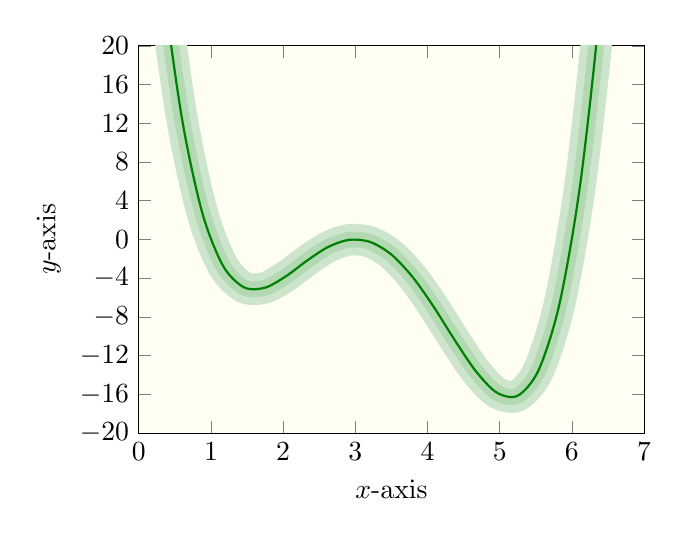
\begin{tikzpicture}
	\begin{axis}[
	xmin = 0, xmax = 7,
	ymin = -20, ymax = 20,
	width = 8cm,
	height = 6.5cm,
	xtick distance = 1,
	ytick distance = 4,
	smooth,
	xlabel=$x$-axis,
	ylabel=$y$-axis,
	set layers,
	]
	\begin{pgfonlayer}{axis background}
	\fill [yellow!5] (0,-20) rectangle (7,20);
	\end{pgfonlayer}
	\addplot[Green!20, domain = 0:7, line width=4mm] {(x-1)*(x-3)^2*(x-6)};
	\addplot[Green!30, domain = 0:7, line width=2mm] {(x-1)*(x-3)^2*(x-6)};
	\addplot[Green, domain = 0:7, thick] {(x-1)*(x-3)^2*(x-6)};
	\end{axis}
	\end{tikzpicture}
\end{document}